\documentclass[tikz,border=5]{standalone}
\usepackage{amsmath}
\usepackage{tikz}
\usepgfmodule{nonlineartransformations}
\usetikzlibrary{curvilinear,patterns,decorations.pathreplacing,spy,calc}
\usepackage{pgfplots}
\usepackage{pgfplotstable}
\usepgfplotslibrary{groupplots}
\pgfplotsset{/pgfplots/table/search path={dat}}

\begin{document}

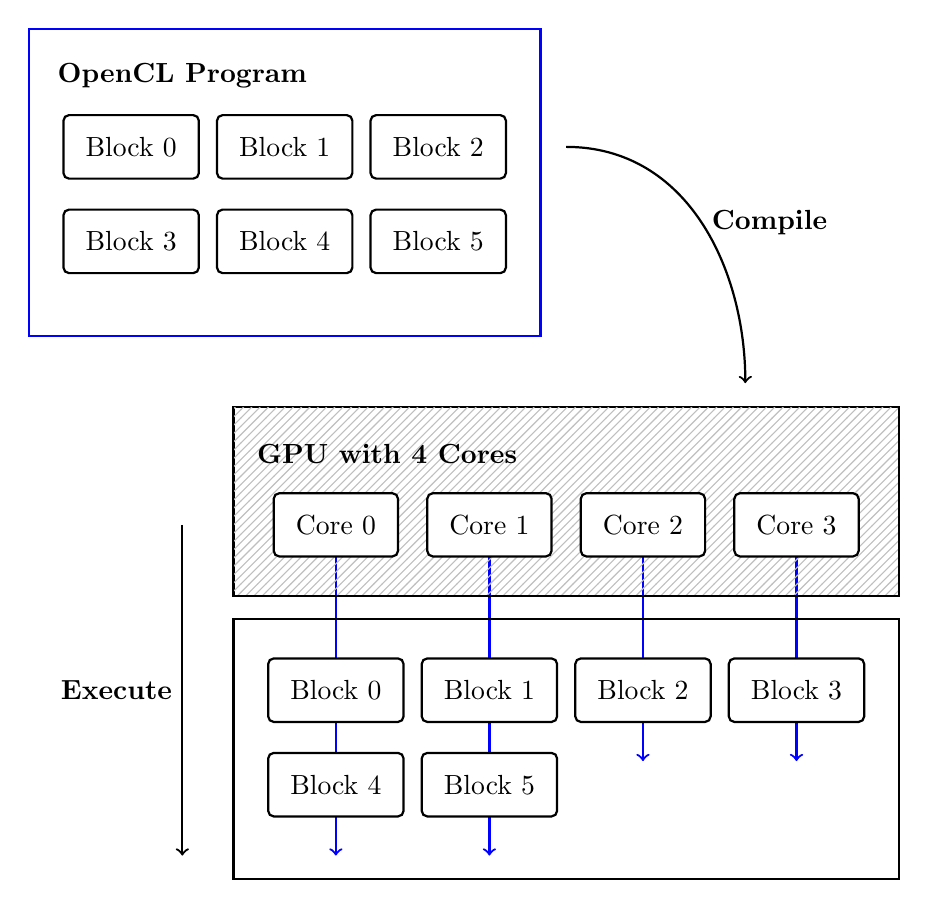
\begin{tikzpicture}[xscale=1.3,yscale=1.2]
\def\block(#1,#2,#3,#4){\node[draw=black,thick,rounded corners=2,inner sep=8,fill=white] (#1) at (#2,#3) [anchor=center] {#4};}


% blocks1
\begin{scope}[shift={(0,7)}]
\draw[thick,blue](-1,-0) rectangle (4,3.25);
\node at (0.5,2.75) {\bf{OpenCL Program}};
\block(E, 0.0, 1, Block 3)
\block(F, 1.5, 1, Block 4)
\block(G, 3.0, 1, Block 5)
\block(E, 0.0, 2, Block 0)
\block(F, 1.5, 2, Block 1)
\block(G, 3.0, 2, Block 2)
\end{scope}

%arrows
\begin{scope}[shift={(2,1.25)}]
\draw[->,thick,blue] (0.0,4) to (0.0,+0.25);
\draw[->,thick,blue] (1.5,4) to (1.5,+0.25); 
\draw[->,thick,blue] (3.0,4) to (3.0,+1.25); 
\draw[->,thick,blue] (4.5,4) to (4.5,+1.25); 
\end{scope}

% gpu
\begin{scope}[shift={(2,5)}]
\draw[thick,black](-1,-0.75) rectangle (5.5,1.25);
\draw[pattern=north east lines,pattern color=lightgray](-1,-0.75) rectangle (5.5,1.25);
\node at (0.5,0.75) {\bf{GPU with 4 Cores}};
\block(A, 0.0, 0, Core 0)
\block(B, 1.5, 0, Core 1)
\block(C, 3.0, 0, Core 2)
\block(E, 4.5, 0, Core 3)
\end{scope}

% blocks2
\begin{scope}[shift={(2,1.25)}]
\draw[thick,black](-1,0) rectangle (5.5,2.75);
\block(A, 0.0, 2, Block 0)
\block(B, 1.5, 2, Block 1)
\block(C, 3.0, 2, Block 2)
\block(E, 4.5, 2, Block 3)
\block(A, 0.0, 1, Block 4)
\block(B, 1.5, 1, Block 5)
\end{scope}

%arrows
\draw[->,black,thick,out=0,in=90] (4.25,9) to node [midway,above,black,anchor=west] {\bf{Compile}} (6,6.5) ;
\draw[->,black,thick] (0.5,5) to node [midway,above,black,anchor=east] {\bf{Execute}} (0.5,1.5) ;

\end{tikzpicture}

\end{document}